\begin{frame}{Applications - Image processing}
    \textbf{Goal} : Facial Feature Extraction\\
    ~\\
    \begin{figure}
        \centering
        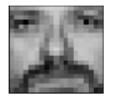
\includegraphics[width=2cm]{../images/face_image.png}
    \end{figure}
    Data matrix : $X\in\real^{p\times n}_+$\\
    \begin{itemize}
        \item $p$ : total number of pixels
        \item $n$ : number of faces
        \item $X(i,j)$ : the gray-level of the $i$-th pixel in the $j$-th face
    \end{itemize}
\end{frame}
    
\begin{frame}{Applications - Image processing}
    \begin{figure}
        \centering
        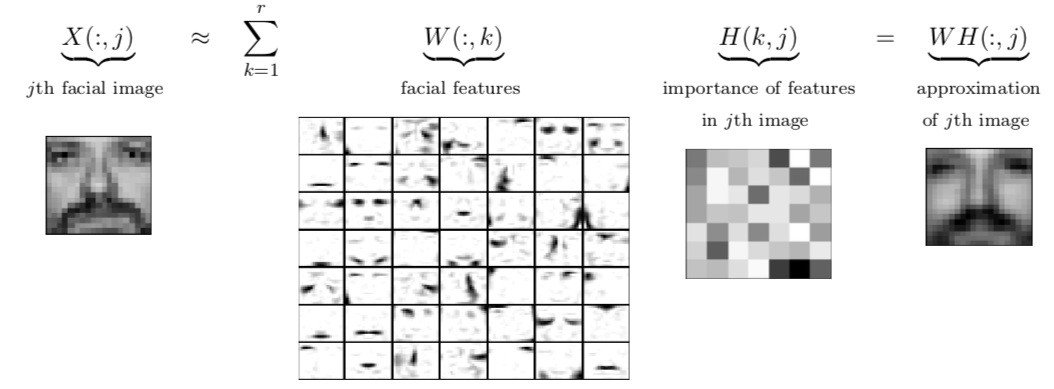
\includegraphics[width=\linewidth]{../images/NMF_app1.png}
    \end{figure}
\end{frame}

\begin{frame}{Applications - Image processing}
    \begin{figure}[h!]
        \centering
        \begin{minipage}{0.45\textwidth}
            \centering
            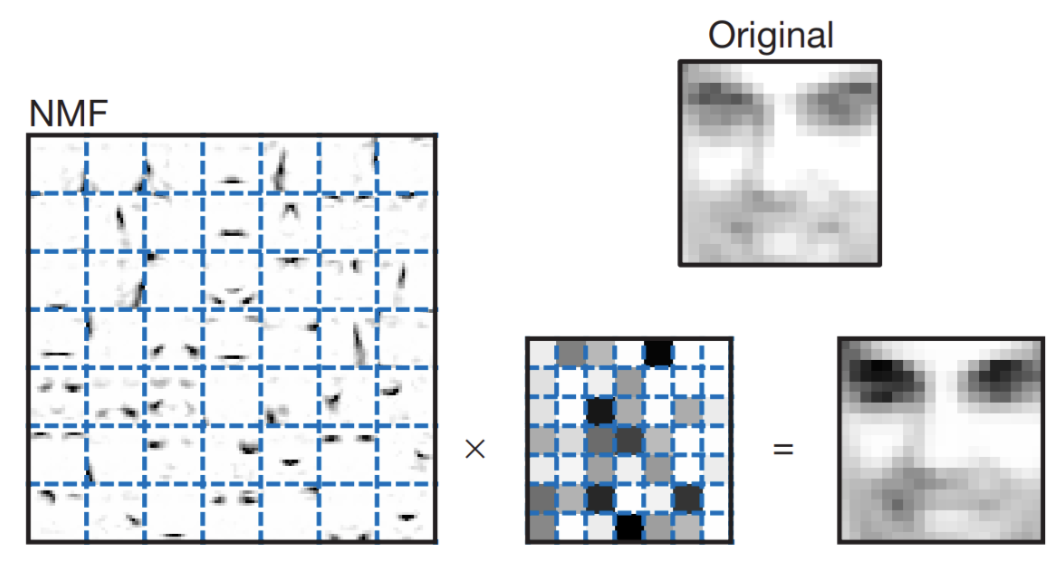
\includegraphics[width=5.3cm]{../images/NMFcomp.png}
            %\caption{NMF decomposition}
            NMF decomposition
        \end{minipage}
        \hfill
        \begin{minipage}{0.45\textwidth}
            \centering
            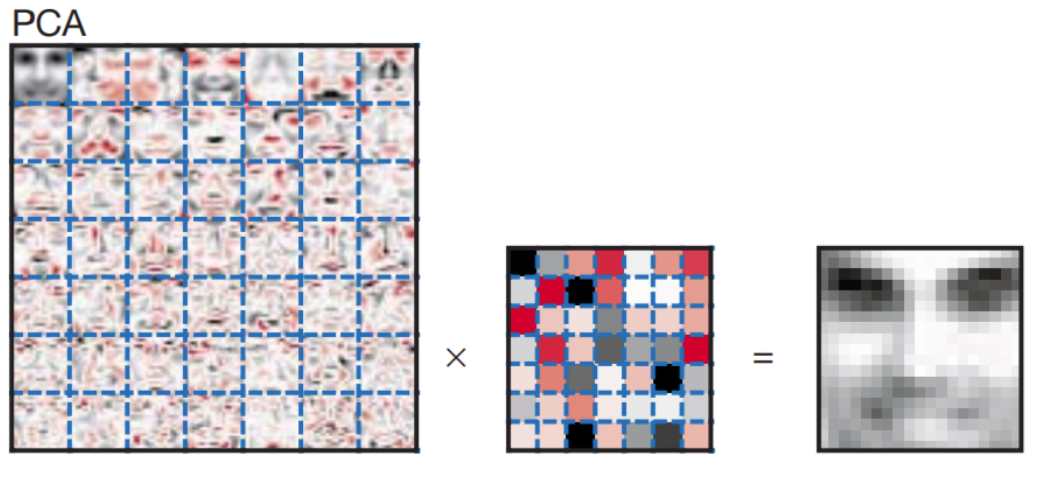
\includegraphics[width=5.5cm]{../images/PCAcomp.png}
            %\caption{PCA decomposition}
            PCA decompostion
        \end{minipage}
    \end{figure}
\end{frame}
\begin{frame}{Applications - Text Mining}
    \textbf{Goal} : Topic Recovery and Document Classification\\
    \vspace{0.7cm}
    Data matrix : $X\in\real^{n\times m}_+$\\
    \begin{itemize}
        \item each column : a document
        \item each line : a word
        \item $X(i,j)$ : number of times the $i$-th word appears in the $j$-th document
    \end{itemize}
    \begin{figure}
        \centering
        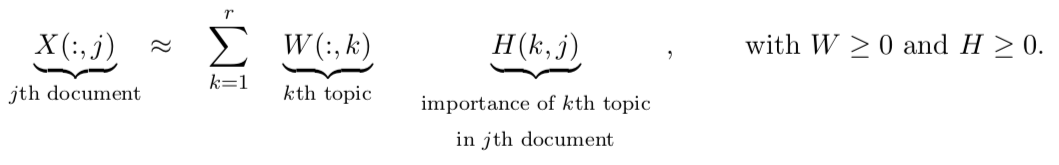
\includegraphics[width=0.9\linewidth]{../images/NMF_app2.png}
    \end{figure}
\end{frame}
\begin{frame}{Applications - Hyperspectral Unmixing}
    \textbf{Goal} :
    \begin{enumerate}
        \item Identify the constitutive materials present in an image
        \item Classify the pixels according to their constitutive materials
    \end{enumerate}
    \vspace{1cm}
    \textbf{Spectral signature} of a pixel: fraction of incident light being reflected by that pixel at different wavelengths\\
    \begin{figure}
        \centering
        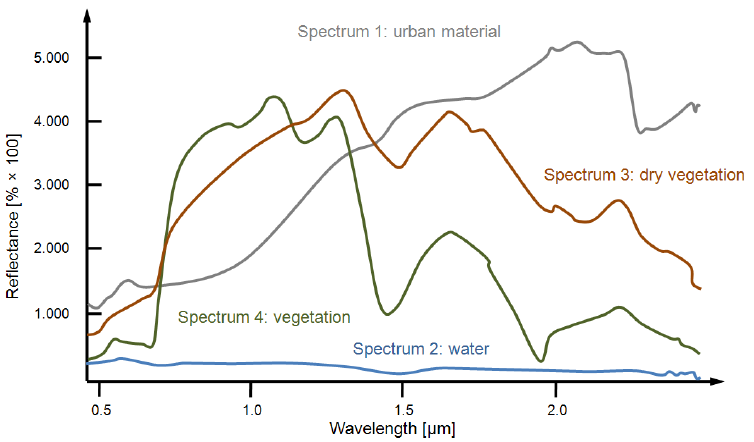
\includegraphics[width=0.65\linewidth]{../images/Spectral-signatures.png}
    \end{figure}
\end{frame}

\begin{frame}{Applications - Hyperspectral Unmixing}
    Data matrix : $X\in\real^{n\times m}$\\
    \begin{itemize}
        \item each column : spectral signature of a pixel
    \end{itemize}
    \begin{figure}
        \centering
        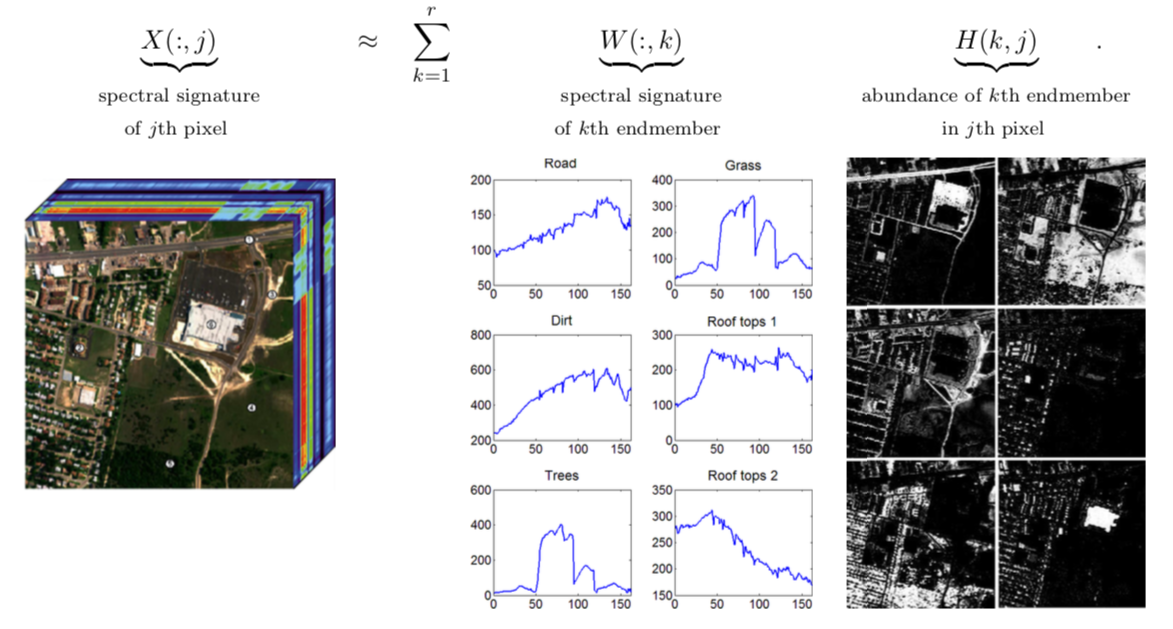
\includegraphics[width=0.85\linewidth]{../images/NMF_app3.png}
    \end{figure}
\end{frame}
